\section{Symulacyjne wyznaczenie odpowiedzi skokowej procesu}

Odpowiedzi skokowych procesu zostały wyznaczone symulacyjnie dla pięciu zmian sygnału sterującego. 
Uwzględnione zostały ograniczenia wartości tego sygnału Umin=0.1, Umax=1.5. 
Początkowa wartość sterowania wynosiła Upp=0.8.

\begin{figure}[H]
    \centering
    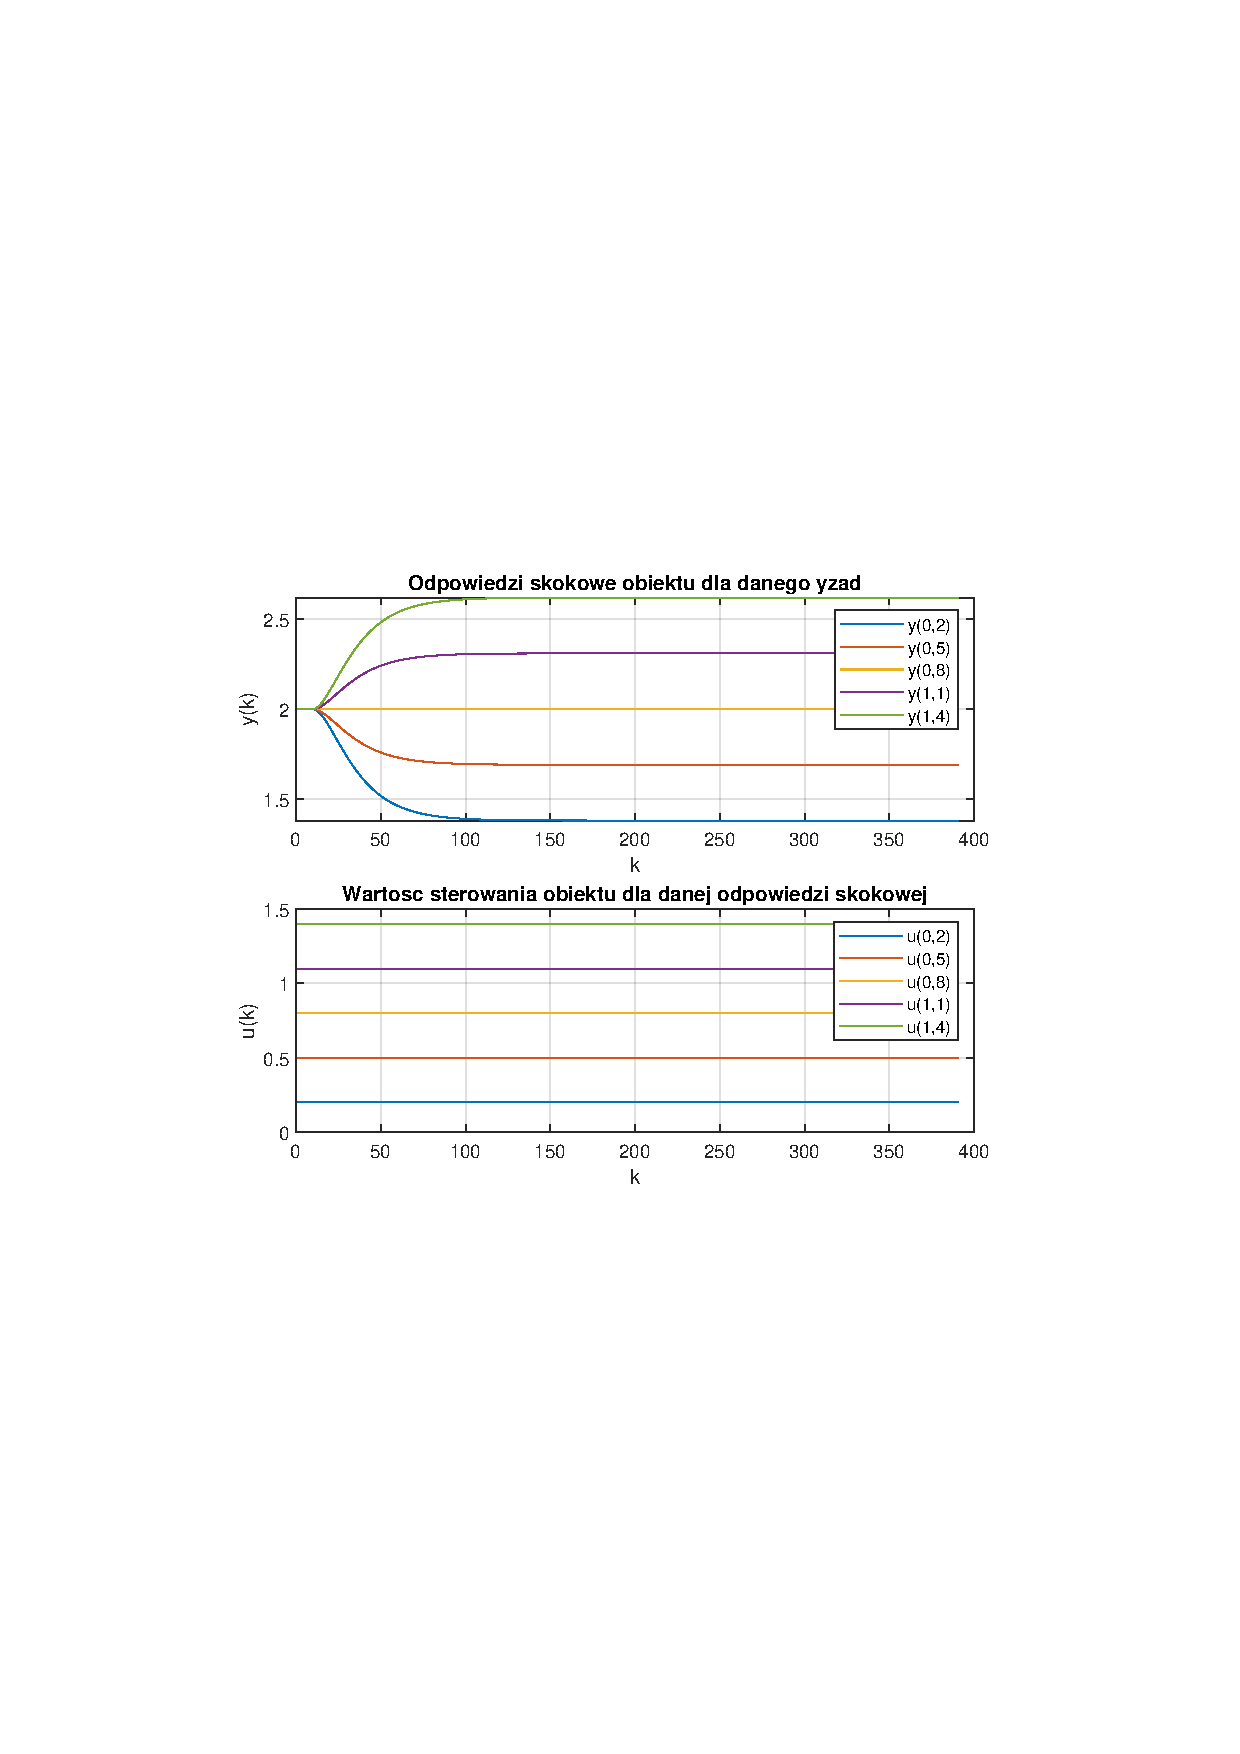
\includegraphics[scale=0.8]{../projekt/zad2/Dane/odp_skok.pdf}
    \caption{ odpSkok }
\end{figure}

Dzięki uzyskanym odpowiedziom skokowym otrzymano charakterystykę statyczną y(u)
\begin{figure}[H]
    \centering
    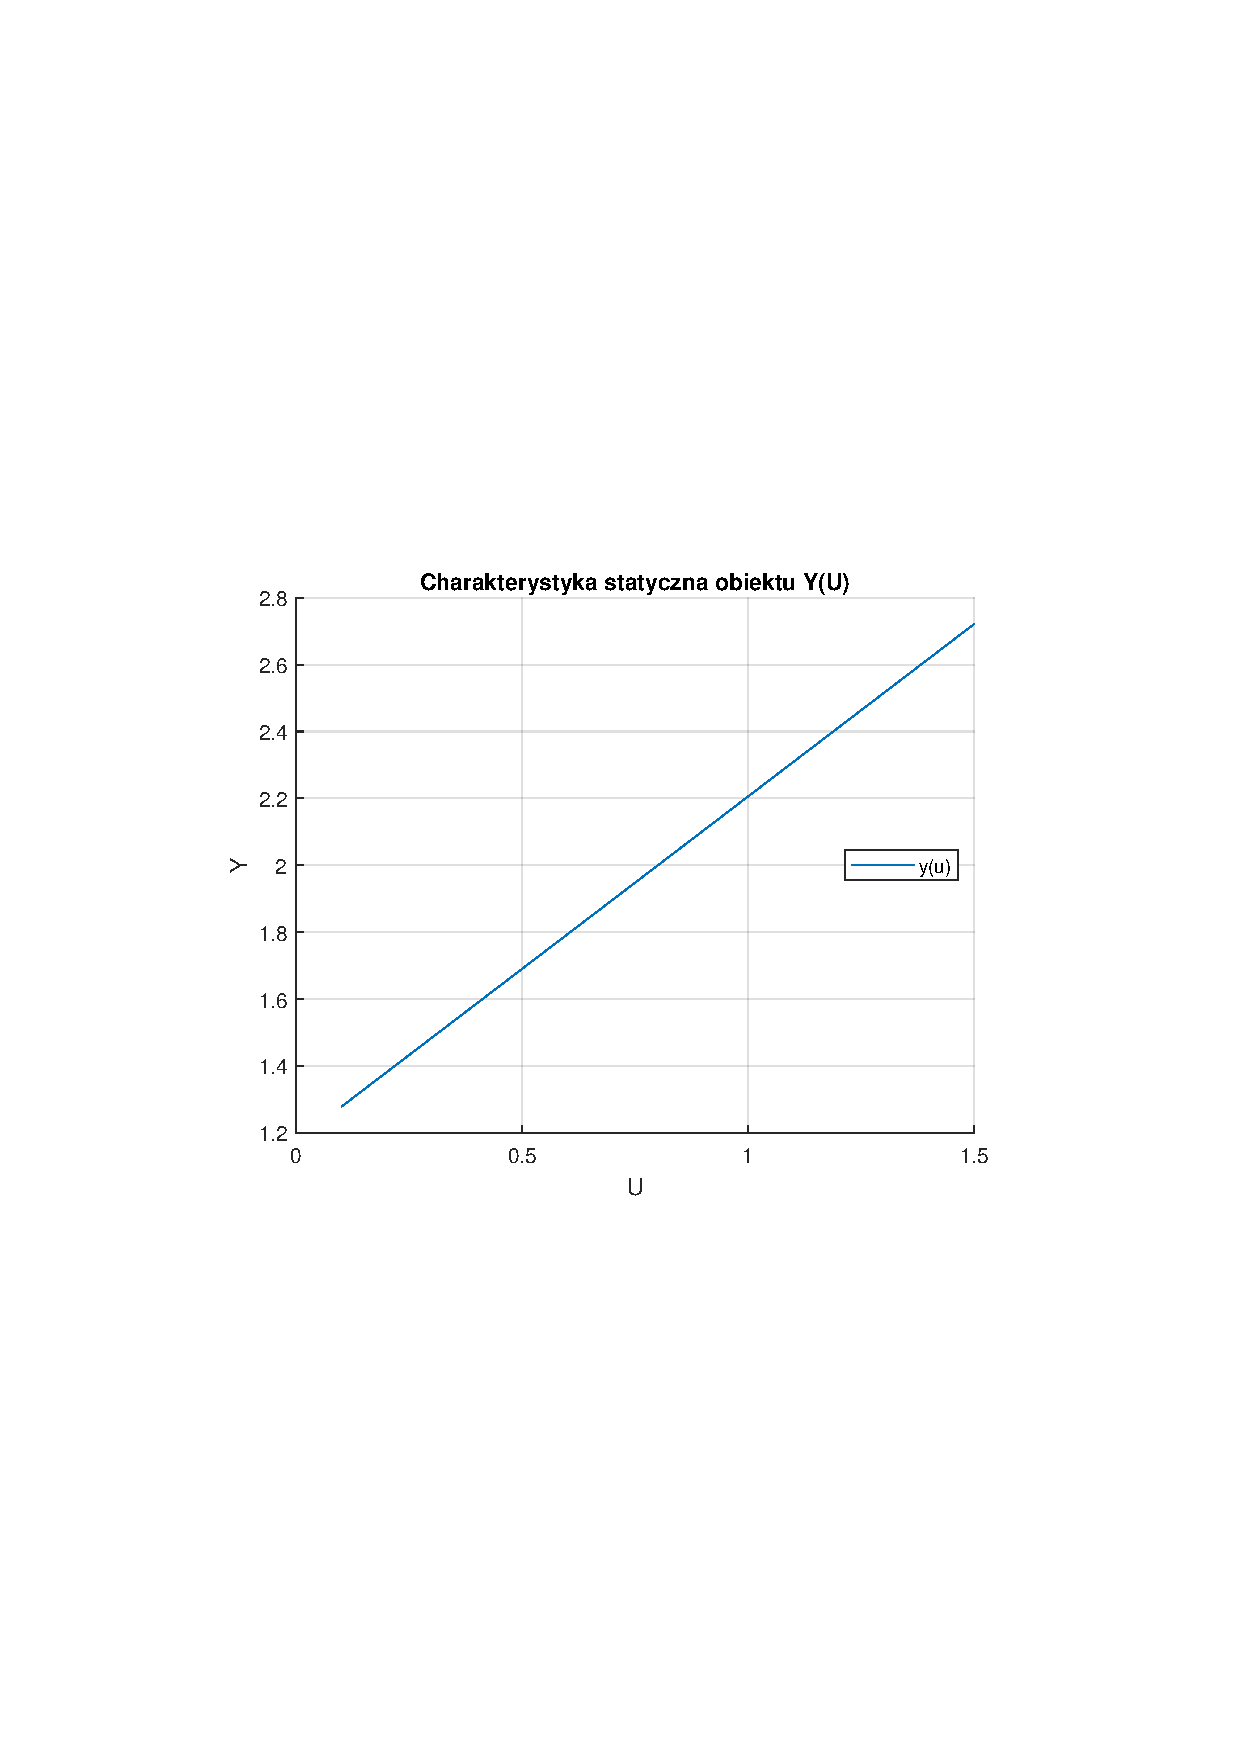
\includegraphics[scale=0.8]{../projekt/zad2/Dane/char_stat.pdf}
    \caption{char stat}
\end{figure}

Wniosek: 
Na podstawie wykresu charakterystyki statycznej można ustalić, 
że właściwości statyczne procesu są liniowe. 
Wzmocnienie statyczne procesu określone zostało dzięki obliczeniu współczynnika nachylenia 
wykresu charakterystyki statycznej, wynosi on K=1.0305.
